% Theorie: Physikalische Grundlagen von Versuch/Messverfahren, Gleichungen ohne Herleitung knapp erklären
\section[Theorie]{Theorie \textnormal{\cite{geiger}}}
\label{sec:theorie}

Geiger-Müller Zählrohre dienen der Detektion ionisierender Strahlung. Da die Nachweiswahrscheinlichkeit für energiereiche Bereiche des
elektromagnetischen Spektrums wie Röntgen- oder Gammastrahlung sehr gering ist, wird hauptsächlich Teilchenstrahlung betrachtet. Diese
kann in Alpha- und Betastrahlung eingeteilt werden: Handelt es sich um Elektronen $(\ce{e-})$ heißt sie $\beta^-$-Strahlung, für Positronen
$(\ce{e+})$ wird sie $\beta^+$-Strahlung genannt. Setzt sie sich dagegen aus $\alpha$-Teilchen zusammen sind damit Heliumkerne
\raisebox{0.085ex}{\scalebox{0.85}{$\left(\ce{^{4}_{2}He}\right)$}} gemeint. Wie Abbildung \ref{fig:formen} zu sehen ist,
existieren vielfältige Bauformen, die sich aber letztendlich eine wesentliche Funktionsweise teilen.

\begin{figure}[H]
	\centering
	\includegraphics[width=0.5\linewidth]{content/grafik/formen.jpg}
	\caption{Verschiedene Bauformen von Geiger-Müller Zählrohren.}
	\label{fig:formen}
\end{figure}

\subsection{Funktionsweise}

Das Geiger-Müller Zählrohr besteht aus einem metallischen Zylinder entlang dessen Achse ein Zähldraht verläuft. Ein Eintrittsfenster aus
Mylar- oder Glimmerfolie verschließt die Röhre, in der sich bei Unterdruck ein mit einem Kohlenwasserstoff versetztes Edelgas befindet.
Zwischen Anodendraht und Kathodenzylinder wird ein radialsymmetrisches elektrisches Feld angelegt.

\begin{figure}[H]
	\centering
	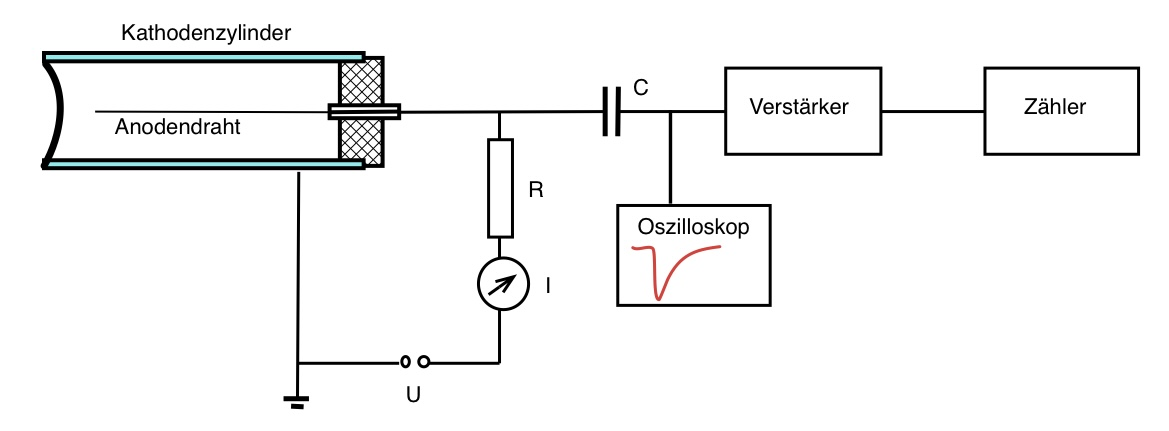
\includegraphics[width=0.8\linewidth]{content/grafik/diagramm.jpg}
	\caption{Schematischer Aufbau des Geiger-Müller Zählrohrs.}
	\label{fig:diagramm}
\end{figure}

Einfallende ionisierende Strahlung produziert im Füllgasgemisch freie Elektronen, die wegen ihrer negativen Ladung zum Zähldraht beschleunigen,
sowie positiv geladene Ionen, die in Richtung Zylinderwand wandern. Diese Ladungsträger können dabei weitere Moleküle ionisieren, sodass sich
Kettenreaktionen ausbilden. Der entstehende Strom fließt über einen Widerstand im Bereich einiger \qty{e6}{\ohm} ab, sodass es bei ausreichender
Stromstärke nahezu instantan zu einem Spannungsabfall kommt. Das Feld wird dadurch abgeschwächt und die Kettenreaktion stoppt. Nach Abfließen der
Ladung nimmt die Feldstärke wieder zu und es kann ein weiterer Ionisationsprozess detektiert werden. Um die Spannungspulse messbar zu machen, ist
dem Zähler noch ein Verstärker vorgeschaltet. Nachzuvollziehen ist dieser Aufbau mithilfe des Blockdiagramms in Abbildung \ref{fig:diagramm}.

\subsection{Funktionsbereiche}

Die Beziehung von Zählrate zu angelegter Spannung heißt Zählrohrcharakteristik und kann graphisch als Kennlinie (Abbildung \ref{fig:kurve})
dargestellt werden. Daran lassen sich verschiedene Bereiche ablesen, in denen jeweils unterschiedliche physikalische Prozesse dominieren.

\begin{figure}[H]
	\centering
	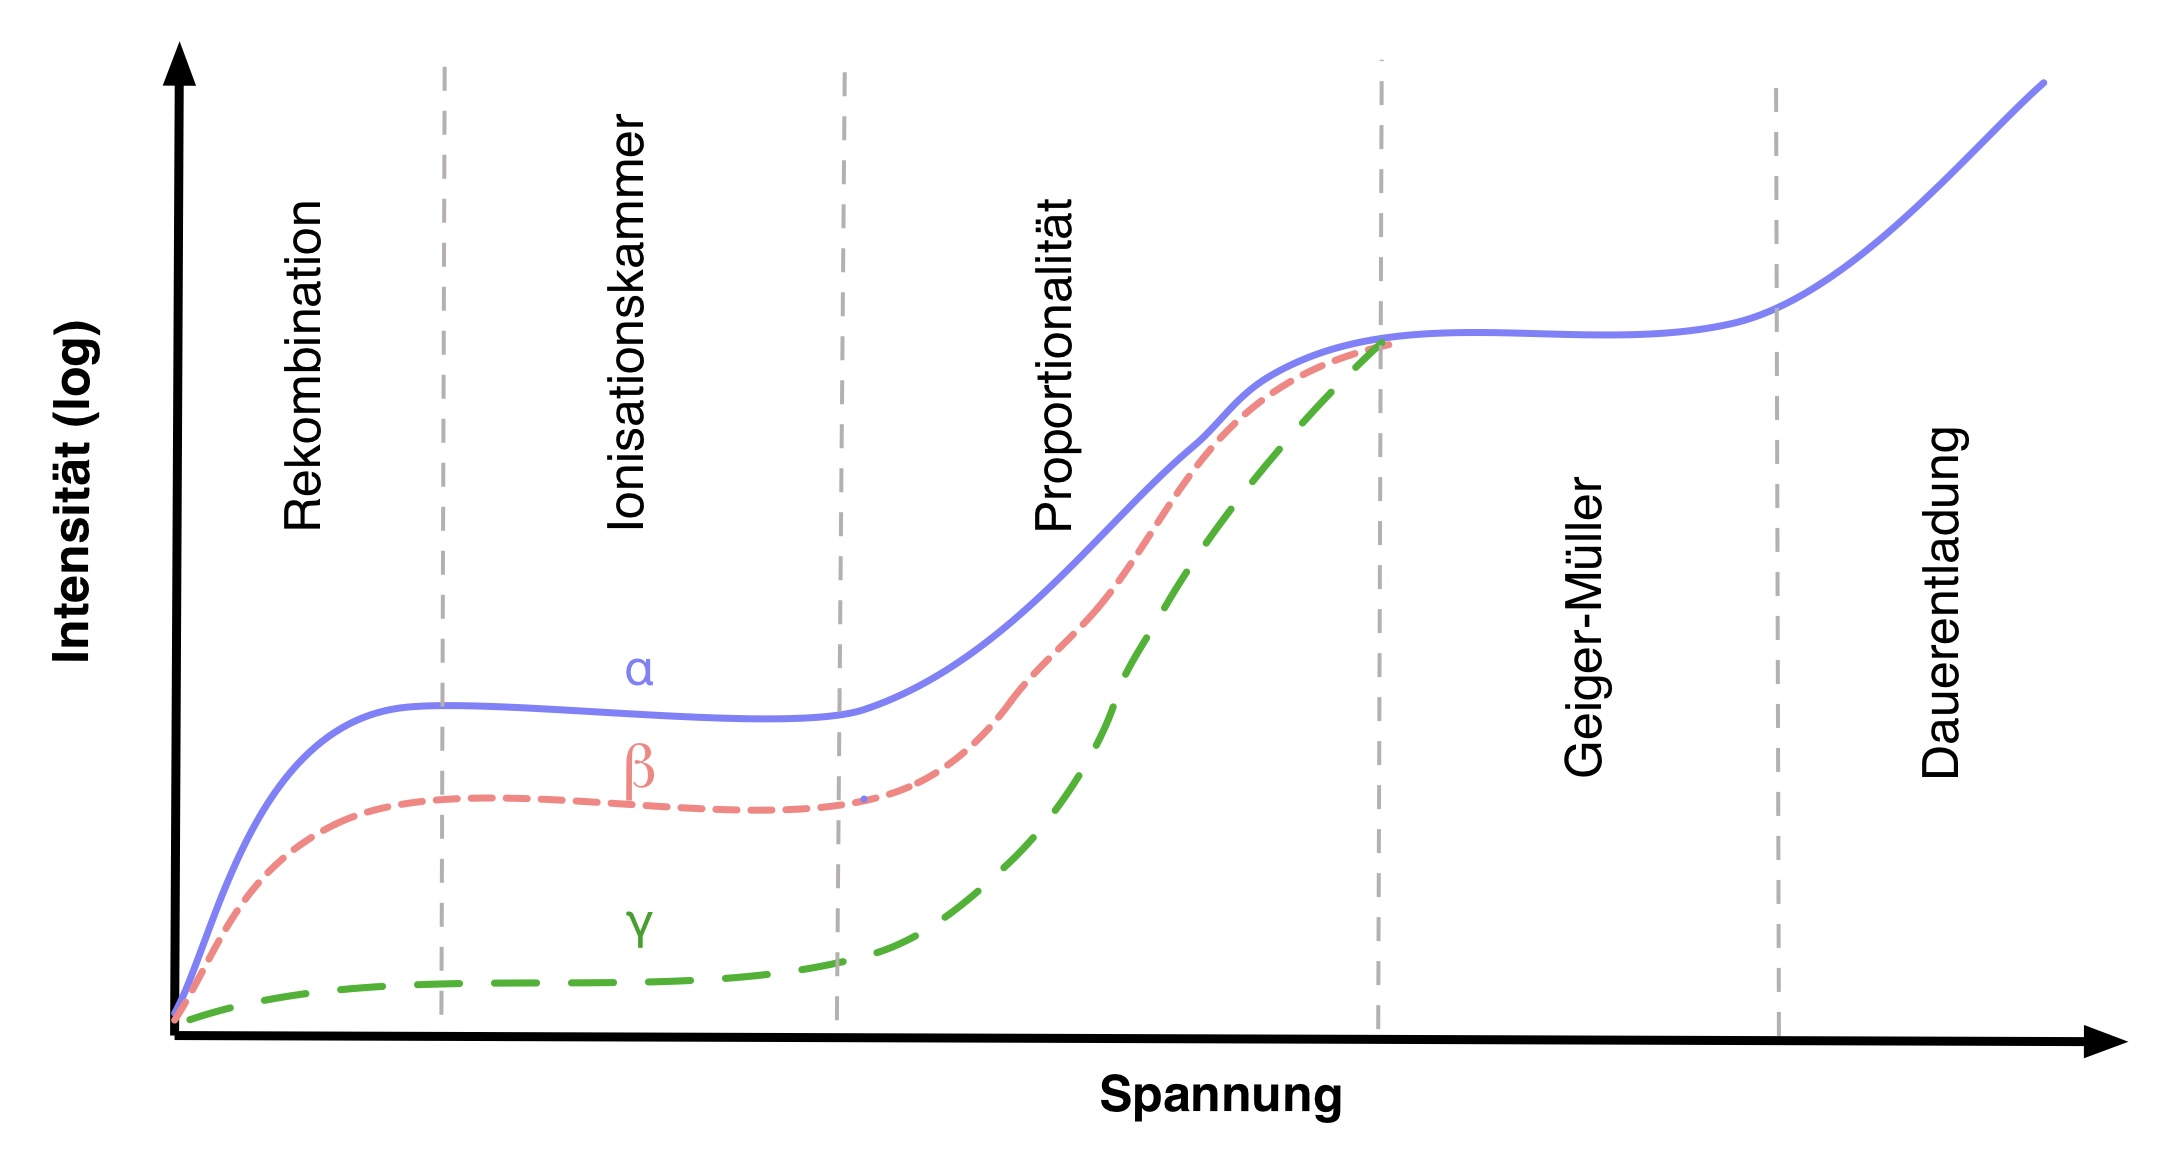
\includegraphics[width=0.7\linewidth]{content/grafik/kurve.jpg}
	\caption{Typische Kennlinie eines Geiger-Müller Zählrohrs.}
	\label{fig:kurve}
\end{figure}

\subsubsection{Charakteristik der Kennlinie}

Die in Abbildung \ref{fig:kurve} eingetragenen Spannungsabschnitte werden \mbox{nun genauer beschrieben:}

\paragraph{Rekombination}

Bei geringen Spannungen rekombinieren sich die Ionisationsprodukte wieder zu neutralen Atomen, sodass sie nicht zum resultierenden Strom beitragen.
Daher kann die Apparatur erst ab einer Mindestspannung Zerfälle nachweisen. Mit zunehmender Spannung wird dieser Einfluss vernachlässigbar gering.

\paragraph{Ionisationskammer}

Alle Ladungsträger erreichen die Elektroden, auf diese Weise stellt sich ein Sättigungsstrom ein. Es handelt sich dabei nur um durch die
Primärstrahlung erzeugte Elektronen und Ionen, da die für sekundäre Ionisationsprozesse notwendige Energie in diesem Spannungsbereich nicht
erreicht wird.

\paragraph{Proportionalität}

Die freigesetzten Elektronen erzeugen durch Stoßionisation weitere Elektronen-Ionen-Paare, lokalisiert um den Anodendraht findet
dieser Prozess aufgrund der hohen Feldstärke lawinenartig statt. Abhängig von Zählrohrspannung, Gasdruck und Gasart, sorgen diese
sogenannten Townsend-Lawinen für Verstärkungsfaktoren in der Ordnung \num{e3}. Der Verlauf ist hier außerdem proportional zum spezifischen
Ionisationsvermögen und erlaubt so eine Unterscheidung der einfallenden Strahlung nach Art und Energie. Dabei erzeugt $\alpha$-Strahlung eine
sehr große Ladung, für $\beta$- und $\gamma$-Strahlung fällt diese geringer aus.

\paragraph{Geiger-Müller}

Weiteres Erhöhen der Spannung sorgt dafür, dass im gesamten Zählrohrvolumen Townsend-Lawinen auftreten. Aufgrund der viel höheren trägen
Masse der Ionen relativ zu den Elektronen, können erstere nicht ausreichend schnell abwandern, sodass sich um den Zähldraht eine abschirmende
Raumladungswolke bildet. Diese verhindert das Auftreten weiterer Lawinen, die Magnitude der Impulse wird so unabhängig von der Strahlungsart
auf den gleichen Wert beschränkt. Der Arbeitspunkt des Geiger-Müller Zählrohrs liegt im ersten Drittel des entstehenden Plateaus.

Im Geiger-Müller Bereich treten zusätzliche Störphänomene auf: Angeregte Gasatome emittieren Photonen, die am Kathodenzylinder Photoelektronen 
erzeugen können, welche wiederum lawinenartig verstärkt werden. Ebenso führen Stöße energetischer Ionen mit der Zylinderwand zur zeitversetzten
Emission von Sekundärelektronen, deren als Nachentladungen bezeichnete Ausgangsimpulse die gemesse Zählrate verfälschen. Zur Mitigation beider
Prozesse kann ein Löschgas aus langkettigen Alkoholmolekülen beigefügt werden, das Photonen absorbiert und Nachentladungsstöße dämpft.

\paragraph{Dauerentladung}

Ansetzen größerer Spannungen führt zum dauerentladungsbedingten exponentiellen Anstieg der Zählrate und zur langfristigen Zerstörung des Zählrohrs. 

\subsubsection{Kennzeichnende Zeitintervalle}

Im Geiger-Müller Betriebsbereich bezeichnet die Totzeit den Zeitraum, welcher zwischen Erreichen des Impulsmaximums und der Registrierung
neuer Impulse liegt. Die Totzeit des Zählrohrs, im weiteren Gebrauch kurz Totzeit genannt, entspricht also der Zeit, welche die isolierende
Raumladungswolke um den Anodendraht benötigt, um sich soweit zu verflüchtigen, dass neue Spannungspulse auftreten. Da die Apparatur jedoch
erst für Impulse ab einer gewissen Amplitude empfindlich ist, kann eine Totzeit des Detektorsystems benannt werden, welche genau um die
Zeit größer ist, die das elektrische Feld braucht, um wieder eine ausreichende Stärke aufzubauen. Dieses Intervall bis zur erneuten Auslösung
der Messgerätschaft heißt weiter Auslösezeit. Da Totzeit und Auslösezeit in guter Näherung zusammenfallen beziehungsweise nicht unabhängig messbar
sind, werden beide Größen als allgemeine Totzeit $\tau$ zusammengefasst. Mit der Erholungszeit $\Tau$ wird noch der Zeitraum ab dem ersten
registrierten neuen Puls bis zur vollständigen Erholung der Spannung auf das Niveau vor dem ursprünglichen Impuls beschrieben.

\begin{figure}[H]
	\centering
	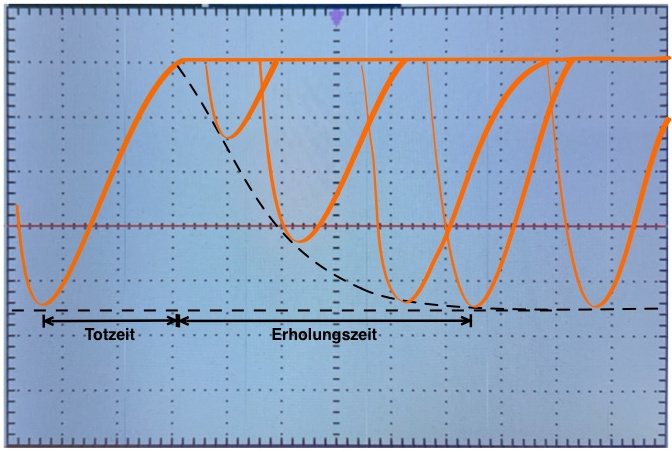
\includegraphics[width=0.5\linewidth]{content/grafik/zeit_soll.jpg}
	\caption{Bestimmung von Totzeit und Erholungszeit am Oszilloskop.}
	\label{fig:zeit_soll}
\end{figure}

\subsubsection{Güte des Plateaus}

Die Wahrscheinlichkeit, dass eine der zuvor beschriebenen Nachentladungen auftritt, steigt mit Detektorspannung und Alter des Zählrohrs. Die
resultierenden zeitversetzten Pulse sorgen somit dafür, dass der Geiger-Müller Bereich nicht konstant verläuft, sondern eine Steigung besitzt.
Diese wird mit
\begin{equation}
	s = \pfrac{\increment N}{N} \, \qty{100}{\percent} \mathbin{/} \qty{100}{\volt}
	\label{eqn:steigung}
\end{equation}
als relative Zählrate $\increment N / N$ pro \qty{100}{\volt} Spannungsänderung definiert und gibt damit ein genormtes Maß der Güte
des Zählrohrs an.

\subsection{Statistik}

Die Zählrate im Geiger-Müller Zählrohr folgt einer Poisson-Verteilung, deren Vorschrift
\begin{equation*}
	P(k, N) = \pfrac{N^k}{k!} \symup e^{-N}
\end{equation*}
lautet. Diese besitzt einen relativen mittleren Fehler
\begin{equation}
	\sigma_\text{rel} = \pfrac{1}{\sqrt{N \,}}
	\label{eqn:relativ}
\end{equation}
und einen statistischen Fehler, der sich direkt über
\begin{equation}
	\sigma = N \sigma_\text{rel} = \sqrt{N \,}
	\label{eqn:statistisch}
\end{equation}
ergibt und die Streubreite einordnet.

